
\documentclass[UTF8,zihao=-4,a4paper]{ctexart}
\usepackage{amsmath,amssymb,mathtools,bm}
\usepackage{geometry,booktabs,longtable,array,enumitem,multicol}
\usepackage{xcolor,tcolorbox,fancyhdr}
\usepackage{float}
\usepackage{tikz}
\usetikzlibrary{arrows.meta,calc,angles,quotes}
\usepackage[font=small,labelfont=bf,labelsep=quad,skip=4pt]{caption}
\setlength{\intextsep}{6pt plus 2pt minus 2pt}
\setlength{\textfloatsep}{8pt plus 2pt minus 2pt}
\usepackage{hyperref}
\usepackage{needspace}
\usepackage{tocloft}
\renewcommand{\cftsecfont}{\bfseries}
\renewcommand{\cftsecpagefont}{\bfseries}
\setlength{\cftbeforesecskip}{5pt}
\setlength{\cftbeforesubsecskip}{0pt}
\setlength{\cftsecindent}{0em}
\setlength{\cftsubsecindent}{2.2em}
\setlength{\cftsecnumwidth}{1.7em}
\setlength{\cftsubsecnumwidth}{2.5em}
\AddToHook{cmd/section/before}{\needspace{6\baselineskip}}
\geometry{left=2.15cm,right=2.15cm,top=2.1cm,bottom=2.2cm}
\setlength{\parindent}{2em}
\setlength{\parskip}{0.25em}
\setlength{\abovedisplayskip}{7pt plus 2pt minus 2pt}
\setlength{\belowdisplayskip}{7pt plus 2pt minus 2pt}
\setlength{\abovedisplayshortskip}{4pt plus 1pt minus 1pt}
\setlength{\belowdisplayshortskip}{4pt plus 1pt minus 1pt}
\setlength{\fboxsep}{3.5pt}
\setlength{\LTpre}{4pt plus 2pt minus 2pt}
\setlength{\LTpost}{4pt plus 2pt minus 2pt}
\setlist[enumerate]{itemsep=0.25em,topsep=0.3em}
\setlist[itemize]{itemsep=0.2em,topsep=0.25em}
\hypersetup{colorlinks=true,linkcolor=black,urlcolor=blue!55!black,citecolor=black,
  pdftitle={圆锥曲线二级结论},pdfauthor={Icelon},pdfsubject={高考数学圆锥曲线二级结论}}
\pagestyle{fancy}
\fancyhf{}
\renewcommand{\headrulewidth}{0.4pt}
\makeatletter
\renewcommand{\sectionmark}[1]{\markboth{\thesection\quad #1}{\thesection\quad #1}}
\renewcommand{\subsectionmark}[1]{}
\makeatother
\fancyhead[L]{\small\sffamily\textcolor{black!70}{圆锥曲线二级结论}}
\fancyhead[R]{\small\sffamily\textcolor{black!70}{\rightmark}}
\fancyfoot[C]{\small\textcolor{black!70}{\thepage}}
\setlength{\headheight}{15pt}
\newtcolorbox{keybox}{colback=blue!3,colframe=blue!45!black,boxrule=0.55pt,arc=1.5mm,left=1.5mm,right=1.5mm,top=1mm,bottom=1mm}
\newtcolorbox{warningbox}{colback=red!3,colframe=red!45!black,boxrule=0.55pt,arc=1.5mm,left=1.5mm,right=1.5mm,top=1mm,bottom=1mm}
\newtcolorbox{derivationbox}{colback=green!3,colframe=green!40!black,boxrule=0.45pt,arc=1.5mm,left=1.5mm,right=1.5mm,top=1mm,bottom=1mm}

% ---------------- 图形样式：试卷风格（黑白细线、无填充） ----------------
\tikzset{
  caxis/.style={->,>=stealth,line width=0.4pt},
  ccurve/.style={line width=0.7pt},
  caux/.style={dashed,line width=0.35pt},
  cseg/.style={line width=0.45pt},
  ctan/.style={line width=0.45pt},
  clab/.style={font=\scriptsize,inner sep=1.2pt},
}
\newcommand{\e}{\mathrm e}
\newcommand{\R}{\mathbb R}
\newcommand{\F}{\mathcal F}
\newcommand{\dd}{\mathrm d}
\newcommand{\abs}[1]{\left|#1\right|}
\newcommand{\norm}[1]{\left\|#1\right\|}
\newcommand{\ds}{\displaystyle}
\title{\bfseries 高考数学圆锥曲线常见二级结论\\[0.4em]\large 通用结论 \;|\; 椭圆 \;|\; 双曲线 \;|\; 抛物线}
\author{高考数学复习资料}
\date{整理版 \quad 2026}

% ---------------- 标题层级：细线条 + 黑体，克制而不喧宾夺主 ----------------
\ctexset{
  section = {
    format     = \sffamily\bfseries\fontsize{15}{19}\selectfont,
    aftername  = \quad,
    beforeskip = 2.0em plus .4em minus .2em,
    afterskip  = .8em plus .2em minus .1em,
    fixskip    = true,
    aftertitle = {\par\vspace{.22em}{\color{black!22}\rule{\textwidth}{.5pt}}\par},
  },
  subsection = {
    format     = \sffamily\bfseries\fontsize{12.6}{15.5}\selectfont,
    aftername  = \quad,
    beforeskip = 1.7em plus .3em minus .1em,
    afterskip  = .4em plus .1em,
    fixskip    = true,
  },
}

\begin{document}

% ================= 封面 =================
\begin{titlepage}
  \thispagestyle{empty}
  \centering
  \vspace*{3.2cm}
  {\sffamily\large 高考数学专题}\par
  \vspace{1.6em}
  {\sffamily\bfseries\fontsize{32}{38}\selectfont 圆锥曲线二级结论}\par
  \vspace{1.4em}
  {\sffamily\large 通用结论 \;·\; 椭圆 \;·\; 双曲线 \;·\; 抛物线}\par
  \vspace{2.6em}
  {\color{black!30}\rule{9.5cm}{0.7pt}}\par
  \vspace{2.2em}
  {\large 面向高考压轴题的公式、条件、推导线索与使用策略}\par
  \vfill
  {\small\textcolor{black!65}{作者：Icelon \qquad 主页：\href{https://Icelon.top}{Icelon.top}}}\par
  \vspace{0.9em}
  {\small\textcolor{black!65}{整理版 \quad 2026}}\par
  \vspace{1.4cm}
\end{titlepage}

% ================= 目录 =================
\pagestyle{empty}
{\footnotesize
\addtocontents{toc}{\protect\footnotesize}
\tableofcontents}
\clearpage

% ================= 正文 =================
\pagenumbering{arabic}
\pagestyle{fancy}

\section{符号约定与三类曲线速查}

\subsection{标准方程、焦点、离心率与准线}

\renewcommand{\arraystretch}{1.45}
\setlength{\tabcolsep}{4pt}
\begin{longtable}{>{\centering\arraybackslash}p{1.5cm}p{4.9cm}p{4.9cm}p{3.9cm}}
\toprule
类型 & 标准方程 & 焦点、离心率 & 准线与渐近线\\
\midrule
椭圆 &
$\dfrac{x^2}{a^2}+\dfrac{y^2}{b^2}=1,\ a>b>0$ &
$F_{1,2}=(\mp c,0)$\newline $c^2=a^2-b^2$，$e=\dfrac ca\in(0,1)$ &
准线 $x=\pm\dfrac{a}{e}=\pm\dfrac{a^2}{c}$；\newline 无渐近线\\
双曲线 &
$\dfrac{x^2}{a^2}-\dfrac{y^2}{b^2}=1,\ a,b>0$ &
$F_{1,2}=(\mp c,0)$\newline $c^2=a^2+b^2$，$e=\dfrac ca>1$ &
准线 $x=\pm\dfrac{a}{e}=\pm\dfrac{a^2}{c}$；\newline 渐近线 $y=\pm\dfrac ba x$\\
抛物线 &
$y^2=2px,\ p>0$ &
$F=(p/2,0)$，$e=1$ &
准线 $x=-p/2$；\newline 对称轴为 $x$ 轴\\
\bottomrule
\end{longtable}
\setlength{\tabcolsep}{6pt}

\begin{figure}[H]
\centering
\begin{tabular}{@{}c@{\hspace{1.2em}}c@{\hspace{1.2em}}c@{}}
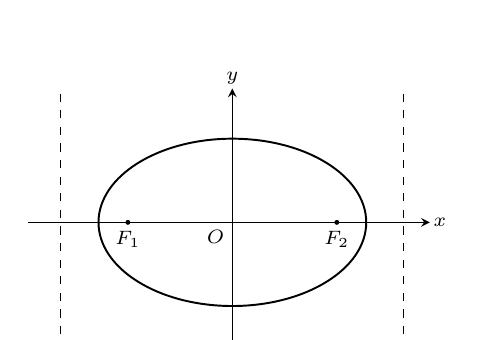
\begin{tikzpicture}[scale=0.85]
  \draw[caxis] (-3.05,0)--(2.95,0) node[clab,right]{$x$};
  \draw[caxis] (0,-1.95)--(0,2.0) node[clab,above]{$y$};
  \draw[ccurve] (0,0) ellipse (2 and 1.25);
  \draw[caux] (-2.562,-1.92)--(-2.562,1.92);
  \draw[caux] (2.562,-1.92)--(2.562,1.92);
  \fill (-1.561,0) circle (1.05pt); \fill (1.561,0) circle (1.05pt);
  \node[clab,below=2pt] at (-1.561,0) {$F_1$};
  \node[clab,below=2pt] at (1.561,0) {$F_2$};
  \node[clab,below left=1.5pt] at (0,0) {$O$};
\end{tikzpicture} &
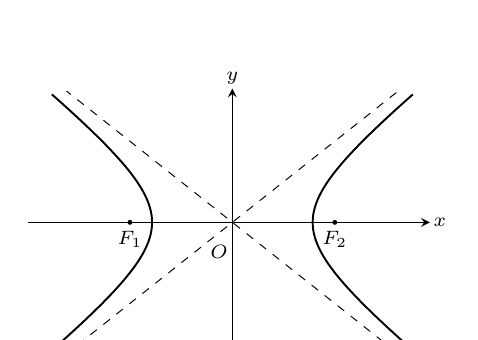
\begin{tikzpicture}[scale=0.85]
  \draw[caxis] (-3.05,0)--(2.95,0) node[clab,right]{$x$};
  \draw[caxis] (0,-1.95)--(0,2.0) node[clab,above]{$y$};
  \begin{scope}
    \clip (-3.02,-1.92) rectangle (2.94,1.96);
    \draw[caux] (-2.9,-2.296)--(2.9,2.296);
    \draw[caux] (-2.9,2.296)--(2.9,-2.296);
  \end{scope}
  \draw[ccurve,domain=-1.45:1.45,samples=90,smooth,variable=\t]
     plot ({1.2*cosh(\t)},{0.95*sinh(\t)});
  \draw[ccurve,domain=-1.45:1.45,samples=90,smooth,variable=\t]
     plot ({-1.2*cosh(\t)},{0.95*sinh(\t)});
  \fill (-1.5305,0) circle (1.05pt); \fill (1.5305,0) circle (1.05pt);
  \node[clab,below=2pt] at (-1.5305,0) {$F_1$};
  \node[clab,below=2pt] at (1.5305,0) {$F_2$};
  \node[clab] at (-0.20,-0.44) {$O$};
\end{tikzpicture} &
\begin{tikzpicture}[scale=0.85]
  \draw[caxis] (-1.05,0)--(2.8,0) node[clab,right]{$x$};
  \draw[ccurve,domain=-2.18:2.18,samples=90,smooth,variable=\t]
     plot ({0.5*\t*\t},{\t});
  \draw[caux] (-0.5,-2.26)--(-0.5,2.3);
  \node[clab,above] at (-0.5,2.3) {$l$};
  \fill (0.5,0) circle (1.05pt);
  \node[clab,below right=1.5pt] at (0.5,0) {$F$};
  \node[clab,below left=1.5pt] at (0,0) {$O$};
\end{tikzpicture}\\
{\scriptsize (a) 椭圆} & {\scriptsize (b) 双曲线} & {\scriptsize (c) 抛物线}
\end{tabular}
\caption{三类标准图形（虚线：椭圆、抛物线为相应准线，双曲线为渐近线）}
\end{figure}

\subsection{几个容易混淆的长度参数}

对椭圆、双曲线，记
\[
\ell=\frac{b^2}{a}\quad\text{（半通径，也称半焦弦参数）},\qquad
d=\frac{b^2}{c}\quad\text{（焦点到对应准线的距离）}.
\]
有
\[
\ell=e\,d,\qquad \text{通径长}=2\ell=\frac{2b^2}{a}.
\]
对抛物线 $y^2=2px$，焦点到准线距离为 $p$，半通径为 $p$，通径长为 $2p$。

\section{圆锥曲线通用二级结论}

\subsection{第二定义：焦点与准线的距离比}

对椭圆、双曲线、抛物线，若 $F$ 为焦点、$l$ 为与该焦点对应的准线，则曲线上点 $P$ 满足
\[
\boxed{\frac{PF}{d(P,l)}=e}.
\]
其中 $e$ 为离心率。椭圆 $0<e<1$，抛物线 $e=1$，双曲线 $e>1$。

\textbf{用途：}题目出现“到焦点距离与到准线距离之比”“定点到定直线距离比为常数”时，优先考虑圆锥曲线第二定义；反过来，也可用第二定义快速求焦点、准线或离心率。

\begin{figure}[H]
\centering
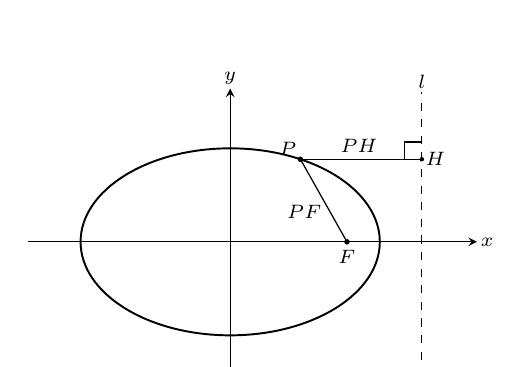
\begin{tikzpicture}[scale=0.95]
  \draw[caxis] (-2.7,0)--(3.3,0) node[clab,right]{$x$};
  \draw[caxis] (0,-1.85)--(0,2.05) node[clab,above]{$y$};
  \draw[ccurve] (0,0) ellipse (2 and 1.25);
  \draw[caux] (2.562,-1.8)--(2.562,2.0) node[clab,above]{$l$};
  \fill (1.561,0) circle (1.05pt);
  \node[clab,below=1.5pt] at (1.561,0) {$F$};
  \coordinate (P) at ({2*cos(62)},{1.25*sin(62)});
  \coordinate (H) at (2.562,{1.25*sin(62)});
  \fill (P) circle (1.05pt) node[clab,above left]{$P$};
  \draw[cseg] (P)--(1.561,0);
  \draw[cseg] (P)--(H);
  \fill (H) circle (0.85pt) node[clab,right]{$H$};
  \coordinate (Ltop) at (2.562,1.95);
  \draw pic[draw,angle radius=2.2mm] {right angle=P--H--Ltop};
  \node[clab] at (0.99,0.40) {$PF$};
  \node[clab,above=1pt] at (1.72,{1.25*sin(62)}) {$PH$};
\end{tikzpicture}
\caption{第二定义：$\frac{PF}{d(P,l)}=e$（$l$ 为与 $F$ 对应的准线）}
\end{figure}

\subsection{顶点连线斜率乘积的轨迹形式（进阶）}
固定 $A_1=(-a,0),A_2=(a,0)$，对不在 $x$ 轴且相关斜率有定义的动点 $P(x,y)$，令
\[
K=k_{PA_1}k_{PA_2}=\frac{y}{x+a}\cdot\frac{y}{x-a}=\frac{y^2}{x^2-a^2}.
\]
则
\[
\boxed{\begin{array}{ll}
K=-1:&x^2+y^2=a^2\quad(\text{圆}),\\[0.25em]
K<0,\ K\ne-1:&\displaystyle\frac{x^2}{a^2}+\frac{y^2}{-Ka^2}=1\quad(\text{椭圆}),\\[0.6em]
K>0:&\displaystyle\frac{x^2}{a^2}-\frac{y^2}{Ka^2}=1\quad(\text{双曲线}).
\end{array}}
\]
\begin{figure}[H]
\centering
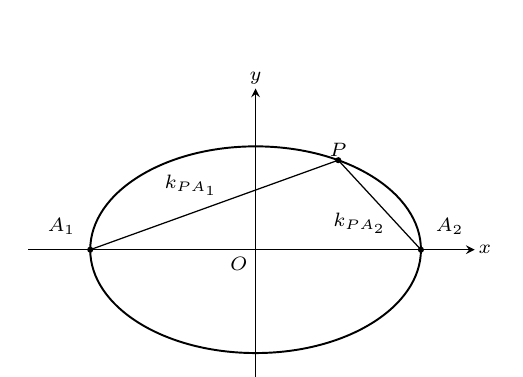
\begin{tikzpicture}[scale=1.05]
  \draw[caxis] (-2.75,0)--(2.65,0) node[clab,right]{$x$};
  \draw[caxis] (0,-1.7)--(0,1.95) node[clab,above]{$y$};
  \draw[ccurve] (0,0) ellipse (2 and 1.25);
  \fill (-2,0) circle (1.05pt); \fill (2,0) circle (1.05pt);
  \node[clab,above left=4pt] at (-2,0) {$A_1$};
  \node[clab,above right=4pt] at (2,0) {$A_2$};
  \coordinate (P) at ({2*cos(60)},{1.25*sin(60)});
  \fill (P) circle (1.05pt) node[clab,above]{$P$};
  \draw[cseg] (P)--(-2,0); \draw[cseg] (P)--(2,0);
  \node[clab] at (-0.78,0.78) {$k_{PA_1}$};
  \node[clab] at (1.26,0.32) {$k_{PA_2}$};
  \node[clab,below left=1.5pt] at (0,0) {$O$};
\end{tikzpicture}
\caption{固定顶点 $A_1,A_2$，动点 $P$ 处两弦斜率之积 $K$ 决定轨迹类型}
\end{figure}

$K=0$ 时方程的代数轨迹退化为 $x$ 轴；但本段预先要求 $P$ 不在 $x$ 轴上，因此该情形不属于允许的动点。这是一种由斜率乘积识别椭圆、圆、双曲线的轨迹模型；它不产生非退化抛物线。上述非退化轨迹还需剔除 $A_1,A_2$（此时相关斜率不存在）。

\subsection{焦半径的坐标表达式}

设 $P(x,y)$ 在曲线上。

\begin{enumerate}
\item \textbf{椭圆：}若 $F_1=(-c,0),F_2=(c,0)$，则
\[
\boxed{PF_1=a+ex,\qquad PF_2=a-ex.}
\]
因此 $PF_1+PF_2=2a$。

\item \textbf{双曲线：}若 $F_1=(-c,0),F_2=(c,0)$，则
\[
\boxed{PF_1=\abs{a+ex},\qquad PF_2=\abs{a-ex}.}
\]
若 $P$ 在右支（$x\ge a$），则 $PF_1=ex+a,\ PF_2=ex-a$，从而
\[
PF_1-PF_2=2a.
\]
若 $P$ 在左支（$x\le-a$），则两焦距的次序相反，距离差的绝对值仍为 $2a$。

\item \textbf{抛物线：}若 $P=(x,y)$ 在 $y^2=2px$ 上，则
\[
\boxed{PF=x+\frac p2=d(P,\ x=-\frac p2).}
\]
即抛物线上任一点到焦点的距离等于它到准线的距离。
\end{enumerate}

\begin{figure}[H]
\centering
\begin{tabular}{@{}c@{\hspace{2em}}c@{}}
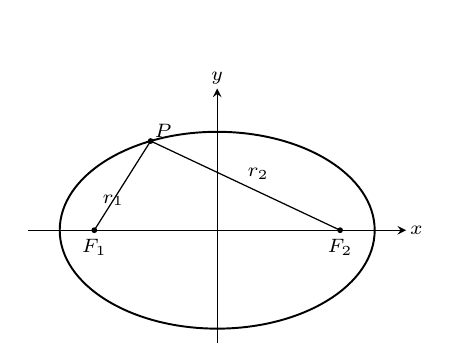
\begin{tikzpicture}[scale=1.0]
  \draw[caxis] (-2.4,0)--(2.4,0) node[clab,right]{$x$};
  \draw[caxis] (0,-1.6)--(0,1.8) node[clab,above]{$y$};
  \draw[ccurve] (0,0) ellipse (2 and 1.25);
  \fill (-1.561,0) circle (1.05pt); \fill (1.561,0) circle (1.05pt);
  \node[clab,below=2pt] at (-1.561,0) {$F_1$};
  \node[clab,below=2pt] at (1.561,0) {$F_2$};
  \coordinate (P) at ({2*cos(115)},{1.25*sin(115)});
  \fill (P) circle (1.05pt) node[clab,above right]{$P$};
  \draw[cseg] (P)--(-1.561,0); \draw[cseg] (P)--(1.561,0);
  \node[clab] at (-1.32,0.38) {$r_1$};
  \node[clab] at (0.52,0.72) {$r_2$};
\end{tikzpicture} &
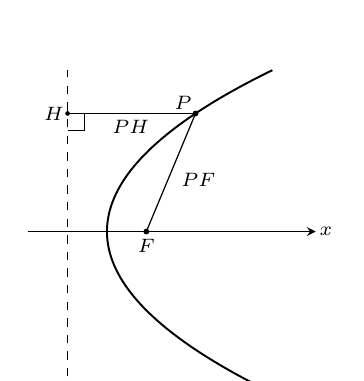
\begin{tikzpicture}[scale=1.0]
  \draw[caxis] (-1.0,0)--(2.65,0) node[clab,right]{$x$};
  \draw[ccurve,domain=-2.05:2.05,samples=90,smooth,variable=\t]
     plot ({0.5*\t*\t},{\t});
  \draw[caux] (-0.5,-2.05)--(-0.5,2.05);
  \coordinate (P) at (1.125,1.5);
  \coordinate (H) at (-0.5,1.5);
  \fill (0.5,0) circle (1.05pt) node[clab,below=1.5pt]{$F$};
  \fill (P) circle (1.05pt) node[clab,above left]{$P$};
  \fill (H) circle (0.85pt) node[clab,left]{$H$};
  \draw[cseg] (P)--(0.5,0); \draw[cseg] (P)--(H);
  \coordinate (Ltop) at (-0.5,1.2);
  \draw pic[draw,angle radius=2.2mm] {right angle=P--H--Ltop};
  \node[clab,below=1pt] at (0.30,1.5) {$PH$};
  \node[clab] at (1.16,0.66) {$PF$};
\end{tikzpicture}\\
{\scriptsize (a) 椭圆} & {\scriptsize (b) 抛物线}
\end{tabular}
\caption{焦半径：椭圆 $r_1+r_2=2a$；抛物线 $PF=d(P,l)$}
\end{figure}

\subsection{参数方程：设点时优先考虑}

\[
\begin{array}{ll}
\text{椭圆：}&P(\theta)=(a\cos\theta,\ b\sin\theta),\\[0.3em]
\text{双曲线：}&P(\theta)=(a\sec\theta,\ b\tan\theta),\quad \cos\theta\ne0,\\[0.3em]
\text{抛物线：}&P(t)=\left(\dfrac p2t^2,\ pt\right),\quad t\in\R.
\end{array}
\]
椭圆参数 $\theta$ 称为离心角；抛物线参数 $t$ 与点的纵坐标满足 $y=pt$。抛物线中，参数法通常比直接设 $(x,y)$ 更简洁。

\subsection{切线方程与极线方程}

设 $P_0(x_0,y_0)$ 为曲线上一点。切线方程如下：
\[
\begin{array}{ll}
\text{椭圆：}&\boxed{\dfrac{xx_0}{a^2}+\dfrac{yy_0}{b^2}=1},\\[0.8em]
\text{双曲线：}&\boxed{\dfrac{xx_0}{a^2}-\dfrac{yy_0}{b^2}=1},\\[0.8em]
\text{抛物线：}&\boxed{yy_0=p(x+x_0)}.
\end{array}
\]
把 $P_0$ 换成任意点 $Q(u,v)$，相应左端的线性式仍定义 $Q$ 关于该二次曲线的\textbf{极线}：
\[
\begin{array}{ll}
\text{椭圆：}&\dfrac{xu}{a^2}+\dfrac{yv}{b^2}=1,\\[0.5em]
\text{双曲线：}&\dfrac{xu}{a^2}-\dfrac{yv}{b^2}=1,\\[0.5em]
\text{抛物线：}&yv=p(x+u).
\end{array}
\]
当 $Q$ 在曲线上时，极线就是该点的切线；当 $Q$ 能作出两条实切线时，极线是两切点连线（切点弦）。

\begin{keybox}
\textbf{极点—极线常用性质}\\
若点 $Q$ 的极线经过点 $P$，则点 $P$ 的极线也经过点 $Q$（互易性）。因此，已知两切点或两切线交点时，可以在“切点弦”和“极线”之间互相转化。
\end{keybox}

\subsection{焦点弦端点处切线的交点（进阶统一性质）}
设 $AB$ 是过焦点 $F$ 的弦，$A,B$ 处切线交于 $T$。由于 $T$ 是弦 $AB$ 的极点，而 $F\in AB$，由极点—极线互易性，$T$ 必在 $F$ 的极线上。对标准形式而言，焦点的极线恰好是对应准线：
\[
\boxed{\begin{array}{ll}
\text{椭圆、双曲线右焦点 }F=(c,0):&x_T=\dfrac{a^2}{c},\\[0.6em]
\text{椭圆、双曲线左焦点 }F=(-c,0):&x_T=-\dfrac{a^2}{c},\\[0.6em]
\text{抛物线焦点 }F=(p/2,0):&x_T=-p/2.
\end{array}}
\]
\begin{figure}[H]
\centering
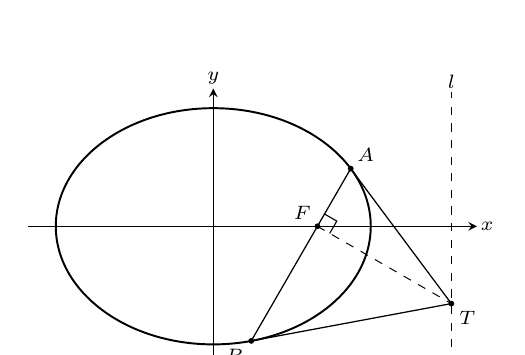
\begin{tikzpicture}[scale=1.0]
  \draw[caxis] (-2.35,0)--(3.35,0) node[clab,right]{$x$};
  \draw[caxis] (0,-1.8)--(0,1.75) node[clab,above]{$y$};
  \draw[ccurve] (0,0) ellipse (2 and 1.5);
  \draw[caux] (3.0237,-1.75)--(3.0237,1.7) node[clab,above]{$l$};
  \coordinate (A) at (1.7456,0.7321);
  \coordinate (B) at (0.4824,-1.4557);
  \coordinate (T) at (3.0237,-0.982);
  \coordinate (Fc) at (1.3229,0);
  \draw[ctan] (A)--(T);
  \draw[ctan] (B)--(T);
  \draw[cseg] (A)--(B);
  \fill (A) circle (1.05pt) node[clab,above right=1pt]{$A$};
  \fill (B) circle (1.05pt) node[clab,below left=1.5pt]{$B$};
  \fill (T) circle (1.05pt) node[clab,below right=1.5pt]{$T$};
  \fill (Fc) circle (1.05pt) node[clab,above left=1pt]{$F$};
  \draw[caux] (Fc)--(T);
  \draw pic[draw,angle radius=1.8mm] {right angle=A--Fc--T};
\end{tikzpicture}
\caption{焦点弦端点处的切线交于 $T$，$T$ 在准线上且 $FT\perp AB$}
\end{figure}

进一步可证，在非退化且 $T$ 为有限点时，$FT\perp AB$。对椭圆、双曲线，若焦点弦恰为长轴或实轴上的顶点弦，端点切线平行，交点在无穷远处；抛物线的轴线与曲线只有一个有限交点，不构成有限焦点弦。

\subsection{直线与圆锥曲线联立：韦达、判别式、弦长}

设直线 $l:y=kx+m$。若交点为 $A(x_1,y_1),B(x_2,y_2)$，则
\[
y_1-y_2=k(x_1-x_2),\qquad
\boxed{AB=\sqrt{1+k^2}\,\abs{x_1-x_2}}.
\]
若联立后得到关于 $x$ 的二次方程 $Ax^2+Bx+C=0$，则
\[
x_1+x_2=-\frac BA,\quad x_1x_2=\frac CA,\quad
\abs{x_1-x_2}=\frac{\sqrt{\Delta}}{\abs A},
\quad \Delta=B^2-4AC.
\]
所以
\[
\boxed{AB=\frac{\sqrt{1+k^2}\sqrt{\Delta}}{\abs A}}.
\]
这里要求 $A\ne0$ 且确有两个有限交点。若直线竖直或二次项系数为零，应回到原方程单独处理。

\subsubsection*{三类曲线的 $y=kx+m$ 速算式}

\textbf{（1）椭圆} $\dfrac{x^2}{a^2}+\dfrac{y^2}{b^2}=1$：
\[
(b^2+a^2k^2)x^2+2a^2kmx+a^2(m^2-b^2)=0.
\]
令 $A_E=b^2+a^2k^2$，则
\[
\boxed{x_1+x_2=-\frac{2a^2km}{A_E},\quad
x_1x_2=\frac{a^2(m^2-b^2)}{A_E}},
\]
\[
\boxed{\Delta_E=4a^2b^2(A_E-m^2)}.
\]
相交于两点的条件为 $m^2<A_E$；相切条件为 $m^2=A_E$。弦长
\[
\boxed{AB=\frac{2ab\sqrt{(1+k^2)(a^2k^2+b^2-m^2)}}{b^2+a^2k^2}}.
\]
特别地，直线 $y=kx+m$ 与椭圆相切当且仅当
\[
\boxed{m^2=a^2k^2+b^2}.
\]

\textbf{（2）双曲线} $\dfrac{x^2}{a^2}-\dfrac{y^2}{b^2}=1$：
\[
(b^2-a^2k^2)x^2-2a^2kmx-a^2(m^2+b^2)=0.
\]
令 $A_H=b^2-a^2k^2$，则在 $A_H\ne0$ 时
\[
\boxed{x_1+x_2=\frac{2a^2km}{A_H},\quad
x_1x_2=-\frac{a^2(m^2+b^2)}{A_H}},
\]
\[
\boxed{\Delta_H=4a^2b^2(m^2+b^2-a^2k^2)}.
\]
弦长
\[
\boxed{AB=\frac{2ab\sqrt{(1+k^2)(m^2+b^2-a^2k^2)}}{\abs{b^2-a^2k^2}}}.
\]
相切条件为
\[
\boxed{m^2=a^2k^2-b^2,\quad a^2k^2>b^2}.
\]
若 $a^2k^2=b^2$，直线平行于渐近线，二次项消失，不能直接套用上面的韦达、弦长式。

\textbf{（3）抛物线} $\dfrac{y^2}{2p}=x$（即 $y^2=2px,\ p>0$）：
\[
k^2x^2+(2km-2p)x+m^2=0\quad(k\ne0),
\]
\[
\boxed{x_1+x_2=\frac{2(p-km)}{k^2},\quad x_1x_2=\frac{m^2}{k^2}},
\qquad
\boxed{\Delta_P=4p(p-2km)}.
\]
两个不同实交点的条件为 $km<p/2$，相切条件为
\[
\boxed{km=p/2}.
\]
两个有限交点的弦长为
\[
\boxed{AB=\frac{2\sqrt{p(p-2km)(1+k^2)}}{k^2}}.
\]
注意：当 $k=0$ 时，直线 $y=m$ 与抛物线只有一个有限交点，不构成通常意义下的有限弦；抛物线的竖直切线是顶点处的 $x=0$。

\subsection{点差法：中点弦的核心来源}

设 $A(x_1,y_1),B(x_2,y_2)$ 是中心在原点的椭圆或双曲线上的两点。将两点分别代入方程并相减：
\[
\frac{x_1^2-x_2^2}{a^2}\pm
\frac{y_1^2-y_2^2}{b^2}=0,
\]
即
\[
\frac{(x_1+x_2)(x_1-x_2)}{a^2}
\pm\frac{(y_1+y_2)(y_1-y_2)}{b^2}=0.
\]
设弦 $AB$ 的中点为 $M(x_0,y_0)$，且相关斜率存在，则
\[
\boxed{\begin{aligned}
\text{椭圆：}\quad&k_{AB}=-\frac{b^2x_0}{a^2y_0},&
k_{AB}k_{OM}&=-\frac{b^2}{a^2};\\[0.3em]
\text{双曲线：}\quad&k_{AB}=\frac{b^2x_0}{a^2y_0},&
k_{AB}k_{OM}&=\frac{b^2}{a^2}.
\end{aligned}}
\]
这就是常见的中点弦公式，可以看作圆中垂径定理在椭圆、双曲线上的推广。

对抛物线 $y^2=2px$，由
\[
y_1^2-y_2^2=2p(x_1-x_2)
\]
可得
\[
\boxed{y_0\,k_{AB}=p},\qquad
\boxed{k_{AB}=\frac{p}{y_0}}.
\]
上述公式在 $y_0=0$、弦斜率不存在等特殊情形下需单独讨论。

\begin{figure}[H]
\centering
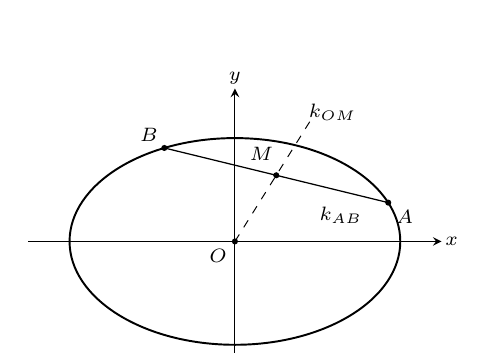
\begin{tikzpicture}[scale=1.05]
  \draw[caxis] (-2.5,0)--(2.5,0) node[clab,right]{$x$};
  \draw[caxis] (0,-1.5)--(0,1.85) node[clab,above]{$y$};
  \draw[ccurve] (0,0) ellipse (2 and 1.25);
  \coordinate (A) at (1.854,0.4695);
  \coordinate (B) at (-0.8536,1.1305);
  \coordinate (M) at (0.5,0.8);
  \draw[cseg] (A)--(B);
  \draw[caux] (0,0)--(0.95,1.52);
  \fill (A) circle (1.05pt) node[clab,below right=1.5pt]{$A$};
  \fill (B) circle (1.05pt) node[clab,above left=1pt]{$B$};
  \fill (M) circle (1.05pt);
  \node[clab] at (0.32,1.06) {$M$};
  \fill (0,0) circle (1.05pt) node[clab,below left=1.5pt]{$O$};
  \node[clab] at (1.28,0.32) {$k_{AB}$};
  \node[clab] at (1.18,1.56) {$k_{OM}$};
\end{tikzpicture}
\caption{点差法：$k_{AB}k_{OM}=-\frac{b^2}{a^2}$（椭圆）}
\end{figure}

\subsection{共轭直径的斜率关系}

对中心在原点的椭圆或双曲线，两条共轭直径的斜率分别为 $k_1,k_2$，则
\[
\boxed{\begin{aligned}
\text{椭圆：}&\quad k_1k_2=-\frac{b^2}{a^2},\\
\text{双曲线：}&\quad k_1k_2=\frac{b^2}{a^2}.
\end{aligned}}
\]
等价地，若共轭半径端点分别为 $P_1(x_1,y_1),P_2(x_2,y_2)$，则
\[
\text{椭圆： }\frac{x_1x_2}{a^2}+\frac{y_1y_2}{b^2}=0;\qquad
\text{双曲线： }\frac{x_1x_2}{a^2}-\frac{y_1y_2}{b^2}=0.
\]
双曲线情形下，与 $OP_1$ 共轭的另一端点 $P_2$ 落在共轭双曲线上。
注意“共轭直径”不是“互相垂直的直径”；只有圆的共轭直径才必然垂直。

\begin{figure}[H]
\centering
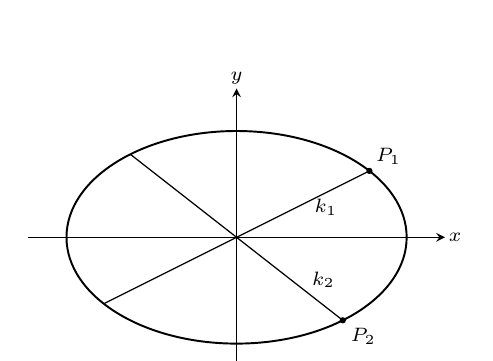
\begin{tikzpicture}[scale=1.08]
  \draw[caxis] (-2.45,0)--(2.45,0) node[clab,right]{$x$};
  \draw[caxis] (0,-1.6)--(0,1.75) node[clab,above]{$y$};
  \draw[ccurve] (0,0) ellipse (2 and 1.25);
  \draw[cseg] (-1.562,-0.781)--(1.562,0.781);
  \draw[cseg] (-1.249,0.976)--(1.249,-0.976);
  \fill (1.562,0.781) circle (1.05pt) node[clab,above right=1pt]{$P_1$};
  \fill (1.249,-0.976) circle (1.05pt) node[clab,below right=1.5pt]{$P_2$};
  \node[clab] at (1.05,0.35) {$k_1$};
  \node[clab] at (1.02,-0.50) {$k_2$};
\end{tikzpicture}
\caption{共轭直径：$k_1k_2=-\frac{b^2}{a^2}$（并不互相垂直）}
\end{figure}

\subsection{两条切线互相垂直：准圆（导圆）}

\begin{enumerate}
\item 椭圆的两条互相垂直的切线交点 $(x,y)$ 满足
\[
\boxed{x^2+y^2=a^2+b^2}.
\]
\item 双曲线 $x^2/a^2-y^2/b^2=1$ 只有在 $a>b$ 时存在实的两条互相垂直切线，其交点满足
\[
\boxed{x^2+y^2=a^2-b^2}.
\]
若 $a\le b$，不存在两条不同的实切线互相垂直。
\item 抛物线 $y^2=2px$ 的两条互相垂直的切线交点轨迹为准线
\[
\boxed{x=-p/2}.
\]
\end{enumerate}
这类轨迹常称为准圆（也叫导圆、蒙日圆）。做题时要先确认曲线类型和实切线存在条件。

\begin{figure}[H]
\centering
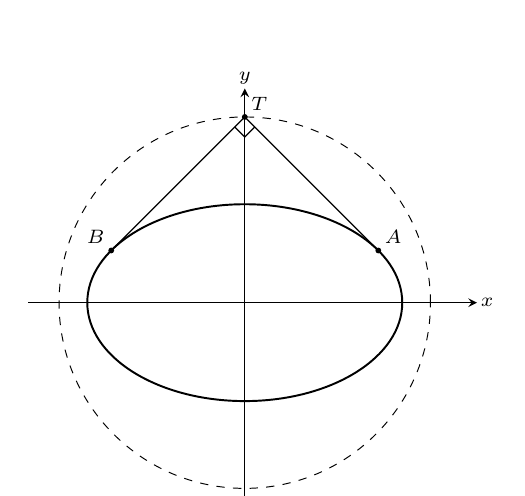
\begin{tikzpicture}[scale=1.0]
  \draw[caxis] (-2.75,0)--(2.95,0) node[clab,right]{$x$};
  \draw[caxis] (0,-2.62)--(0,2.72) node[clab,above]{$y$};
  \draw[dashed,line width=0.35pt] (0,0) circle (2.3585);
  \draw[ccurve] (0,0) ellipse (2 and 1.25);
  \coordinate (T) at (0,2.3585);
  \coordinate (A) at (1.6962,0.6625);
  \coordinate (B) at (-1.6962,0.6625);
  \draw[ctan] (T)--(A);
  \draw[ctan] (T)--(B);
  \fill (T) circle (1.05pt) node[clab,above right=1pt]{$T$};
  \fill (A) circle (1.05pt) node[clab,above right=1pt]{$A$};
  \fill (B) circle (1.05pt) node[clab,above left=1pt]{$B$};
  \draw pic[draw,angle radius=1.8mm] {right angle=A--T--B};
\end{tikzpicture}
\caption{两条互相垂直的切线：交点 $T$ 的轨迹是圆 $x^2+y^2=a^2+b^2$（虚线）}
\end{figure}

\subsection{定比分点点差法（中点弦的推广）}

设 $A(x_1,y_1),B(x_2,y_2)$ 在
\[
\frac{x^2}{a^2}\pm\frac{y^2}{b^2}=1
\]
上，点 $P$ 满足 $\overrightarrow{AP}=\lambda\overrightarrow{PB}$，且 $\lambda\ne-1$。则
\[
x_1+\lambda x_2=(1+\lambda)x_P,\qquad
y_1+\lambda y_2=(1+\lambda)y_P.
\]
由 $A,B$ 的曲线方程相减可得
\[
\boxed{
\frac{(1+\lambda)x_P(x_1-\lambda x_2)}{a^2}
\pm
\frac{(1+\lambda)y_P(y_1-\lambda y_2)}{b^2}
=1-\lambda^2.}
\]
当 $\lambda=1$ 时就是中点弦点差法。若题目给出内分比、定比分点或某点在弦上的位置，这个式子常能避免完整求出两个交点。

\begin{figure}[H]
\centering
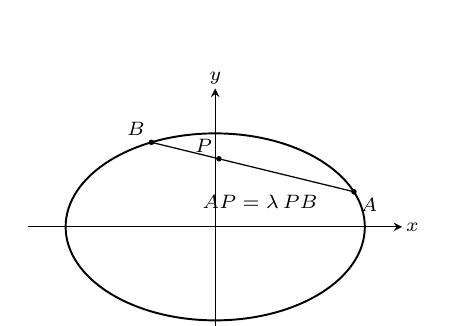
\begin{tikzpicture}[scale=0.95]
  \draw[caxis] (-2.5,0)--(2.5,0) node[clab,right]{$x$};
  \draw[caxis] (0,-1.5)--(0,1.85) node[clab,above]{$y$};
  \draw[ccurve] (0,0) ellipse (2 and 1.25);
  \coordinate (A) at (1.854,0.4695);
  \coordinate (B) at (-0.8536,1.1305);
  \coordinate (P) at (0.0489,0.9102);
  \draw[cseg] (A)--(B);
  \fill (A) circle (1.05pt) node[clab,below right=1pt]{$A$};
  \fill (B) circle (1.05pt) node[clab,above left=1pt]{$B$};
  \fill (P) circle (1.05pt) node[clab,above left=1pt]{$P$};
  \node[clab] at (0.60,0.34) {$AP=\lambda\,PB$};
\end{tikzpicture}
\caption{定比分点：$P$ 在弦 $AB$ 上且 $\overrightarrow{AP}=\lambda\overrightarrow{PB}$}
\end{figure}

\subsection{焦点弦长度：统一表达式}

设过焦点的直线与曲线交于两个有限点 $A,B$，该直线与对称轴（椭圆长轴、双曲线实轴、抛物线轴）的夹角为 $\theta$。令半通径为 $\ell$，则三类曲线均满足
\[
\boxed{AB=\frac{2\ell}{\abs{1-e^2\cos^2\theta}}.}
\]
其中
\[
\ell=
\begin{cases}
b^2/a,&\text{椭圆或双曲线},\\
p,&\text{抛物线 }y^2=2px.
\end{cases}
\]
具体为：
\[
\begin{array}{ll}
\text{椭圆：}&\displaystyle AB=\frac{2b^2/a}{1-e^2\cos^2\theta},\\[0.7em]
\text{双曲线：}&\displaystyle AB=\frac{2b^2/a}{\abs{1-e^2\cos^2\theta}},\\[0.7em]
\text{抛物线：}&\displaystyle AB=\frac{2p}{\sin^2\theta}\quad(\sin\theta\ne0).
\end{array}
\]
双曲线若 $e^2\cos^2\theta=1$，焦点弦所在直线平行于渐近线方向，不能得到两个有限交点；若小于 $1$，交点在同一支；若大于 $1$，交点分居两支。抛物线若 $\theta=0$，轴线与抛物线只有一个有限交点，不构成有限焦点弦。

\begin{figure}[H]
\centering
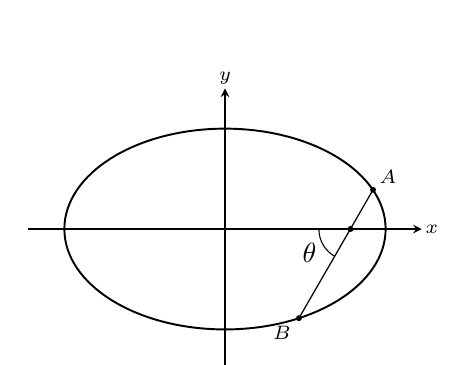
\begin{tikzpicture}[scale=1.02]
  \draw[caxis] (-2.45,0)--(2.45,0) node[clab,right]{$x$};
  \draw[caxis] (0,-1.85)--(0,1.75) node[clab,above]{$y$};
  \draw[ccurve] (0,0) ellipse (2 and 1.25);
  \coordinate (A) at (1.8429,0.4883);
  \coordinate (B) at (0.9203,-1.1098);
  \coordinate (F) at (1.561,0);
  \draw[cseg] (A)--(B);
  \fill (A) circle (1.05pt) node[clab,above right=1pt]{$A$};
  \fill (B) circle (1.05pt) node[clab,below left=1.5pt]{$B$};
  \fill (F) circle (1.05pt);
  \coordinate (X) at (0.9,0);
  \draw pic[draw,angle radius=4mm,"$\theta$",angle eccentricity=1.5] {angle=X--F--B};
\end{tikzpicture}
\caption{焦点弦：$\theta$ 为弦与长轴的夹角，$AB=\frac{2b^2/a}{1-e^2\cos^2\theta}$}
\end{figure}

\subsection{韦达常用对称式}

若 $x_1,x_2$ 是一元二次方程的两根，记 $S=x_1+x_2,\ P=x_1x_2$，则
\[
\begin{aligned}
(x_1-x_2)^2&=S^2-4P,\\
x_1^2+x_2^2&=S^2-2P,\\
x_1^3+x_2^3&=S^3-3PS,\\
\frac1{x_1}+\frac1{x_2}&=\frac SP\quad(P\ne0),\\
\frac{x_1}{x_2}+\frac{x_2}{x_1}&=\frac{S^2}{P}-2\quad(P\ne0).
\end{aligned}
\]
若表达式不对称（如 $x_1/x_2$、$2x_1+x_2$），不要强行套韦达。可尝试交换根、利用已知几何关系，或令 $x_1=u+v,\ x_2=u-v$。

\section{椭圆}

以下均以
\[
\mathcal E:\quad \frac{x^2}{a^2}+\frac{y^2}{b^2}=1,\quad a>b>0,\quad c^2=a^2-b^2,\quad e=\frac ca
\]
为准。

\subsection{焦半径、范围与焦点三角形}

设 $P(x,y)\in\mathcal E$，左右焦点为 $F_1=(-c,0),F_2=(c,0)$。由 §2.3 的焦半径公式可得
\[
\boxed{a-c\le PF_i\le a+c}.
\]
两个端点分别在长轴顶点处取得。

设 $\theta=\angle F_1PF_2$，$r_1=PF_1,r_2=PF_2$。由余弦定理和 $r_1+r_2=2a$ 可得
\[
\boxed{r_1r_2=b^2\sec^2\frac{\theta}{2}},
\qquad
\boxed{S_{\triangle F_1PF_2}=b^2\tan\frac{\theta}{2}}.
\]
这两个式子适用于非退化焦点三角形。

\begin{figure}[H]
\centering
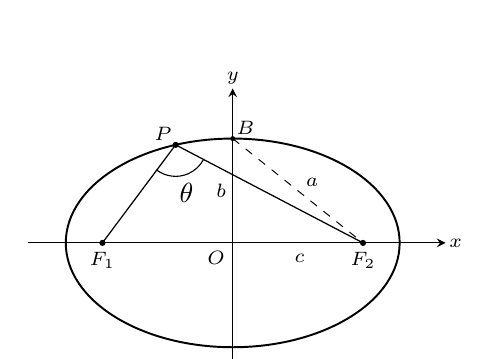
\begin{tikzpicture}[scale=1.06]
  \draw[caxis] (-2.45,0)--(2.55,0) node[clab,right]{$x$};
  \draw[caxis] (0,-1.55)--(0,1.85) node[clab,above]{$y$};
  \draw[ccurve] (0,0) ellipse (2 and 1.25);
  \coordinate (P) at ({2*cos(110)},{1.25*sin(110)});
  \coordinate (F1) at (-1.561,0);
  \coordinate (F2) at (1.561,0);
  \draw[cseg] (P)--(F1); \draw[cseg] (P)--(F2);
  \draw[caux] (0,1.25)--(F2);
  \fill (P) circle (1.05pt) node[clab,above left]{$P$};
  \fill (F1) circle (1.05pt);
  \fill (F2) circle (1.05pt);
  \fill (0,1.25) circle (0.85pt) node[clab,above right]{$B$};
  \node[clab,below=2pt] at (F1) {$F_1$};
  \node[clab,below=2pt] at (F2) {$F_2$};
  \node[clab,below left=1.5pt] at (0,0) {$O$};
  \draw pic[draw,angle radius=4mm,"$\theta$",angle eccentricity=1.55] {angle=F1--P--F2};
  \node[clab,left=1pt] at (0,0.62) {$b$};
  \node[clab] at (0.95,0.72) {$a$};
  \node[clab] at (0.80,-0.18) {$c$};
\end{tikzpicture}
\caption{焦点三角形与 $a,b,c$：$r_1r_2=b^2\sec^2\frac{\theta}{2}$，$S=b^2\tan\frac{\theta}{2}$}
\end{figure}

\subsection{焦点弦：长度、倒数和、焦比}

过焦点 $F$ 的直线与椭圆交于 $A,B$，直线与长轴方向夹角为 $\theta$，令 $r_1=AF,r_2=BF$。由 §2.12 的焦点弦长公式可得
\[
\boxed{\frac1{AF}+\frac1{BF}=\frac{2a}{b^2}},
\qquad
\boxed{AF\cdot BF=\frac{b^4/a^2}{1-e^2\cos^2\theta}}.
\]
若 $\lambda=AF/BF$，则
\[
\boxed{e\abs{\cos\theta}=\frac{\abs{\lambda-1}}{\lambda+1}}.
\]
又由 §2.12 可得
\[
\boxed{\frac{2b^2}{a}\le AB\le 2a}.
\]
最短焦点弦为通径（垂直于长轴，端点为 $(c,\pm b^2/a)$），最长焦点弦为长轴。

\subsection{参数点、切线、法线与弦}

设 $P(\theta)=(a\cos\theta,b\sin\theta)$。

\textbf{切线：}
\[
\boxed{\frac{x\cos\theta}{a}+\frac{y\sin\theta}{b}=1}.
\]

\textbf{法线：}
\[
\boxed{a x\sin\theta-b y\cos\theta=c^2\sin\theta\cos\theta}.
\]
若用一般点 $P(x_0,y_0)$ 表示，切线斜率为 $-b^2x_0/(a^2y_0)$，法线斜率为 $a^2y_0/(b^2x_0)$（分母非零时）。

若 $A,B$ 的离心角分别为 $u,v$，弦 $AB$ 的方程为
\[
\boxed{
\frac{x}{a}\cos\frac{u+v}{2}
+\frac{y}{b}\sin\frac{u+v}{2}
=\cos\frac{u-v}{2}.}
\]
由两条切线（离心角 $u,v$）相交得到的交点 $T$ 为
\[
\boxed{
T\left(
\frac{a\cos\frac{u+v}{2}}{\cos\frac{u-v}{2}},
\frac{b\sin\frac{u+v}{2}}{\cos\frac{u-v}{2}}
\right)}
\]
（分母不为零时）。

\subsection{拉格朗日恒等式与三角形面积上界（进阶）}
设 $A(x_1,y_1),B(x_2,y_2)$ 是椭圆上的两点，则
\[
\boxed{1=\left(\frac{x_1x_2}{a^2}+\frac{y_1y_2}{b^2}\right)^2
+\frac{(x_1y_2-x_2y_1)^2}{a^2b^2}}.
\]
又 $S_{\triangle OAB}=\dfrac12\abs{x_1y_2-x_2y_1}$，所以
\[
\boxed{S_{\triangle OAB}\le\frac{ab}{2}}.
\]
等号当且仅当 $\dfrac{x_1x_2}{a^2}+\dfrac{y_1y_2}{b^2}=0$，即 $OA,OB$ 为共轭半径方向。此式常用于两点在椭圆上、求三角形面积最值或证明定值。

\begin{figure}[H]
\centering
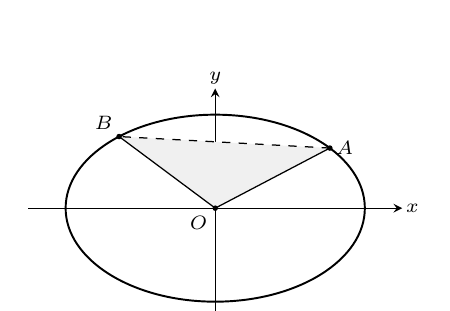
\begin{tikzpicture}[scale=0.95]
  \draw[caxis] (-2.5,0)--(2.5,0) node[clab,right]{$x$};
  \draw[caxis] (0,-1.55)--(0,1.6) node[clab,above]{$y$};
  \fill[black!6] (0,0)--(1.5321,0.8035)--(-1.2856,0.9576)--cycle;
  \draw[ccurve] (0,0) ellipse (2 and 1.25);
  \draw[cseg] (0,0)--(1.5321,0.8035);
  \draw[cseg] (0,0)--(-1.2856,0.9576);
  \draw[cseg,dashed] (1.5321,0.8035)--(-1.2856,0.9576);
  \fill (1.5321,0.8035) circle (1.05pt) node[clab,right=1pt]{$A$};
  \fill (-1.2856,0.9576) circle (1.05pt) node[clab,above left=1pt]{$B$};
  \fill (0,0) circle (1.05pt) node[clab,below left=1.5pt]{$O$};
\end{tikzpicture}
\caption{$OA,OB$ 为共轭半径时 $S_{\triangle OAB}$ 最大，等于 $\frac{ab}{2}$}
\end{figure}

\subsection{焦点三角形内心轨迹（进阶）}

设 $P(x,y)$ 在椭圆上，$I$ 为三角形 $F_1PF_2$ 的内心。利用内心的边长加权坐标公式可得
\[
\boxed{I=\left(ex,\frac{e}{1+e}y\right)}.
\]
因此内心轨迹为椭圆
\[
\boxed{
\frac{x_I^2}{a^2e^2}
+\frac{(1+e)^2y_I^2}{b^2e^2}=1.}
\]
当 $P$ 取长轴端点时三角形退化，故轨迹应看作上述椭圆挖去长轴上的两个顶点。

\subsection{椭圆光学性质}

从一个焦点发出的光线经椭圆反射后，反射光线经过另一个焦点。解析几何中可用“切线与两条焦半径所成角相等”理解。若题目出现反射、入射角等关键词，可优先考虑切线方向或法线方向。

\section{双曲线}

以下均以
\[
\mathcal H:\quad \frac{x^2}{a^2}-\frac{y^2}{b^2}=1,\quad a,b>0,\quad c^2=a^2+b^2,\quad e=\frac ca
\]
为准。

\subsection{焦半径、两支与焦点三角形}

设 $P(x,y)$ 在右支，$F_1=(-c,0),F_2=(c,0)$。由 §2.3 的焦半径公式，$PF_1-PF_2=2a$；左支上两焦距的次序相反，但距离差的绝对值仍为 $2a$。右支上近焦距的最小值为 $c-a$，远焦距的最小值为 $c+a$。

设 $\theta=\angle F_1PF_2$，$r_1=PF_1,r_2=PF_2$，则
\[
\boxed{r_1r_2=b^2\csc^2\frac{\theta}{2}},
\qquad
\boxed{S_{\triangle F_1PF_2}=b^2\cot\frac{\theta}{2}}.
\]
适用于 $P$ 位于右支或左支的非退化焦点三角形。

\subsection{渐近线：距离、垂足与切线截距}

渐近线为
\[
y=\pm\frac ba x.
\]
焦点到任一渐近线的距离为
\[
\boxed{b}.
\]
若 $P(x,y)$ 在双曲线上，$P$ 到两条渐近线的距离分别为 $d_1,d_2$，则
\[
\boxed{d_1d_2=\frac{a^2b^2}{c^2}}.
\]
证明思路：两条渐近线可写为 $bx\mp ay=0$，点到直线距离相乘，再利用 $x^2/a^2-y^2/b^2=1$。

\begin{figure}[H]
\centering
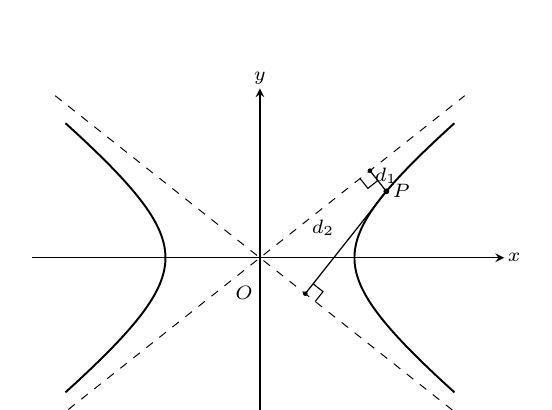
\begin{tikzpicture}[scale=1.0]
  \draw[caxis] (-2.9,0)--(3.1,0) node[clab,right]{$x$};
  \draw[caxis] (0,-2.1)--(0,2.15) node[clab,above]{$y$};
  \begin{scope}
    \clip (-2.95,-2.05) rectangle (3.05,2.1);
    \draw[caux] (-2.6,-2.058)--(2.6,2.058);
    \draw[caux] (-2.6,2.058)--(2.6,-2.058);
  \end{scope}
  \draw[ccurve,domain=-1.35:1.35,samples=60,smooth,variable=\t]
     plot ({1.2*cosh(\t)},{0.95*sinh(\t)});
  \draw[ccurve,domain=-1.35:1.35,samples=60,smooth,variable=\t]
     plot ({-1.2*cosh(\t)},{0.95*sinh(\t)});
  \coordinate (P) at (1.6049,0.8437);
  \coordinate (H1) at (1.3971,1.1061);
  \coordinate (H2) at (0.5760,-0.4560);
  \fill (P) circle (1.05pt) node[clab,right=1pt]{$P$};
  \draw[cseg] (P)--(H1);
  \draw[cseg] (P)--(H2);
  \fill (H1) circle (0.85pt); \fill (H2) circle (0.85pt);
  \coordinate (Q1) at (0.5,0.396);
  \coordinate (Q2) at (1.6,-1.267);
  \draw pic[draw,angle radius=1.6mm] {right angle=P--H1--Q1};
  \draw pic[draw,angle radius=1.6mm] {right angle=P--H2--Q2};
  \node[clab] at (1.60,1.04) {$d_1$};
  \node[clab] at (0.80,0.38) {$d_2$};
  \node[clab] at (-0.20,-0.44) {$O$};
\end{tikzpicture}
\caption{双曲线上点 $P$ 到两渐近线的距离之积 $d_1d_2=\frac{a^2b^2}{c^2}$}
\end{figure}

\textbf{切线与渐近线的中点性质：}过双曲线上点 $P$ 的切线与两条渐近线分别交于 $M,N$，则
\[
\boxed{P\text{ 是 }MN\text{ 的中点}.}
\]
因此，已知切点或切线截距时，可用中点关系快速建立坐标联系。

\begin{figure}[H]
\centering
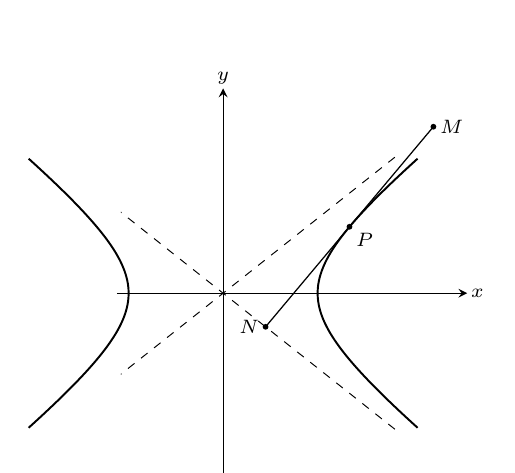
\begin{tikzpicture}[scale=1.0]
  \draw[caxis] (-1.35,0)--(3.1,0) node[clab,right]{$x$};
  \draw[caxis] (0,-2.45)--(0,2.6) node[clab,above]{$y$};
  \begin{scope}
    \clip (-1.3,-2.4) rectangle (3.05,2.55);
    \draw[caux] (-2.2,-1.742)--(2.2,1.742);
    \draw[caux] (-2.2,1.742)--(2.2,-1.742);
  \end{scope}
  \draw[ccurve,domain=-1.35:1.35,samples=60,smooth,variable=\t]
     plot ({1.2*cosh(\t)},{0.95*sinh(\t)});
  \draw[ccurve,domain=-1.35:1.35,samples=60,smooth,variable=\t]
     plot ({-1.2*cosh(\t)},{0.95*sinh(\t)});
  \coordinate (P) at (1.6049,0.8437);
  \coordinate (M) at (2.6706,2.1143);
  \coordinate (N) at (0.5392,-0.4269);
  \draw[ctan] (M)--(N);
  \fill (P) circle (1.05pt) node[clab,below right=1pt]{$P$};
  \fill (M) circle (1.05pt) node[clab,right=1pt]{$M$};
  \fill (N) circle (1.05pt) node[clab,left=1pt]{$N$};
\end{tikzpicture}
\caption{切线交两渐近线于 $M,N$，切点 $P$ 恰为 $MN$ 的中点}
\end{figure}

\subsection{焦点弦：同支与异支必须区分}

过焦点的直线与双曲线交于两个有限点 $A,B$，与实轴方向夹角为 $\theta$。由 §2.12 的焦点弦长公式可知，两交点的位置取决于 $e^2\cos^2\theta$ 与 $1$ 的大小关系：
\begin{itemize}
\item 若 $e^2\cos^2\theta<1$，两交点在同一支，且
\[
\boxed{\frac1{AF}+\frac1{BF}=\frac{2a}{b^2}}.
\]
\item 若 $e^2\cos^2\theta>1$，两交点分居两支，且
\[
\boxed{\abs{\frac1{AF}-\frac1{BF}}=\frac{2a}{b^2}}.
\]
\item 若 $e^2\cos^2\theta=1$，直线平行于渐近线方向，不能把它当作普通的有限焦点弦。
\end{itemize}
\begin{figure}[H]
\centering
\begin{tabular}{@{}c@{\hspace{2em}}c@{}}
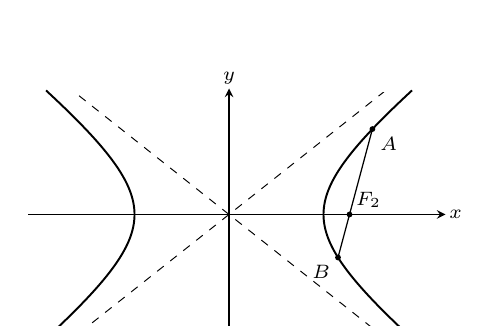
\begin{tikzpicture}[scale=1.0]
  \draw[caxis] (-2.55,0)--(2.75,0) node[clab,right]{$x$};
  \draw[caxis] (0,-1.55)--(0,1.6) node[clab,above]{$y$};
  \begin{scope}
    \clip (-2.5,-1.5) rectangle (2.7,1.55);
    \draw[caux] (-2.4,-1.900)--(2.4,1.900);
    \draw[caux] (-2.4,1.900)--(2.4,-1.900);
  \end{scope}
  \draw[ccurve,domain=-1.28:1.28,samples=70,smooth,variable=\t]
     plot ({1.2*cosh(\t)},{0.95*sinh(\t)});
  \draw[ccurve,domain=-1.28:1.28,samples=70,smooth,variable=\t]
     plot ({-1.2*cosh(\t)},{0.95*sinh(\t)});
  \coordinate (A) at (1.8211,1.0844);
  \coordinate (B) at (1.3842,-0.5462);
  \coordinate (F2) at (1.5305,0);
  \draw[cseg] (A)--(B);
  \fill (A) circle (1.05pt) node[clab,below right=1.5pt]{$A$};
  \fill (B) circle (1.05pt) node[clab,below left=1.5pt]{$B$};
  \fill (F2) circle (1.05pt) node[clab,above right=1pt]{$F_2$};
\end{tikzpicture} &
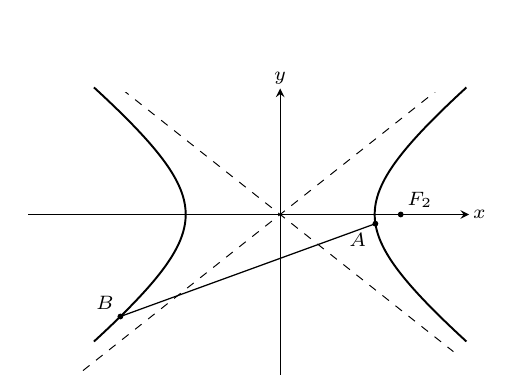
\begin{tikzpicture}[scale=1.0]
  \draw[caxis] (-3.2,0)--(2.4,0) node[clab,right]{$x$};
  \draw[caxis] (0,-2.2)--(0,1.6) node[clab,above]{$y$};
  \begin{scope}
    \clip (-3.15,-2.15) rectangle (2.35,1.55);
    \draw[caux] (-3.0,-2.375)--(2.2,1.742);
    \draw[caux] (-3.0,2.375)--(2.2,-1.742);
  \end{scope}
  \draw[ccurve,domain=-1.3:1.3,samples=60,smooth,variable=\t]
     plot ({1.2*cosh(\t)},{0.95*sinh(\t)});
  \draw[ccurve,domain=-1.3:1.3,samples=60,smooth,variable=\t]
     plot ({-1.2*cosh(\t)},{0.95*sinh(\t)});
  \coordinate (A) at (1.2091,-0.1170);
  \coordinate (B) at (-2.0295,-1.2957);
  \coordinate (F2) at (1.5305,0);
  \draw[cseg] (A)--(B);
  \fill (A) circle (1.05pt) node[clab,below left=2pt]{$A$};
  \fill (B) circle (1.05pt) node[clab,above left=1pt]{$B$};
  \fill (F2) circle (1.05pt) node[clab,above right=1pt]{$F_2$};
\end{tikzpicture}\\
{\scriptsize (a) 同支：$e^2\cos^2\theta<1$} & {\scriptsize (b) 异支：$e^2\cos^2\theta>1$}
\end{tabular}
\caption{双曲线焦点弦：两交点在同支或异支时结论不同}
\end{figure}

这一部分是双曲线最容易误用的结论：不能不看分支就把椭圆的倒数和公式照搬过来。

\subsection{共轭双曲线}

共轭双曲线为
\[
\boxed{\frac{y^2}{b^2}-\frac{x^2}{a^2}=1},
\]
二者有相同的渐近线和相同的半焦距 $c=\sqrt{a^2+b^2}$，但原双曲线的焦点在 $x$ 轴上，共轭双曲线的焦点在 $y$ 轴上，切勿混淆焦点坐标。

\subsection{双曲线双线性恒等式（进阶）}
设 $A(x_1,y_1),B(x_2,y_2)$ 是双曲线上的两点，则
\[
\boxed{\left(\frac{x_1x_2}{a^2}-\frac{y_1y_2}{b^2}\right)^2
-\frac{(x_1y_2-x_2y_1)^2}{a^2b^2}=1}.
\]
因此
\[
\boxed{S_{\triangle OAB}=\frac{ab}{2}
\sqrt{\left(\frac{x_1x_2}{a^2}-\frac{y_1y_2}{b^2}\right)^2-1}}.
\]
它把面积转化为点积型表达式，适合处理双曲线上两动点与原点构成的三角形面积问题。

\subsection{焦点三角形内心轨迹（进阶）}

设 $P$ 在双曲线右支且不取顶点，$I$ 为三角形 $F_1PF_2$ 的内心，则
\[
\boxed{x_I=a}.
\]
即右支对应的焦点三角形内心轨迹是直线 $x=a$ 上的开线段（$-b<y<b$）；若 $P$ 在左支，则内心轨迹是 $x=-a$ 上的对应线段。该结论仅针对焦点三角形的内心，不能误认为是垂心、重心或外心轨迹。

\subsection{双曲线的反射性质}

双曲线在一点处的切线具有焦点反射性质：从一个焦点发出的光线经反射后，其反向延长线经过另一个焦点。处理相关题目时要注意“反向延长线”，这与椭圆的真实反射路径不同。

\section{抛物线}

以下均以
\[
\mathcal P:\quad y^2=2px,\quad p>0,\quad F=(p/2,0),\quad l:x=-p/2
\]
为准。设参数点 $P(t)=\left(\dfrac p2t^2,pt\right)$。

\subsection{切线、法线与两切线交点}

\textbf{参数点 $P(t)$ 处的切线：}
\[
\boxed{ty=x+\frac p2t^2}.
\]
\textbf{参数点 $P(t)$ 处的法线：}
\[
\boxed{y=-tx+pt+\frac p2t^3}.
\]
\textbf{两条切线的交点：}参数分别为 $t_1,t_2$ 的两条切线交于
\[
\boxed{T\left(\frac p2t_1t_2,\ \frac p2(t_1+t_2)\right)}.
\]
因此，两条切线互相垂直当且仅当
\[
\frac1{t_1}\cdot\frac1{t_2}=-1
\iff t_1t_2=-1,
\]
此时交点 $T$ 满足 $x_T=-p/2$，即在准线上。

\begin{figure}[H]
\centering
\begin{tabular}{@{}c@{\hspace{2em}}c@{}}
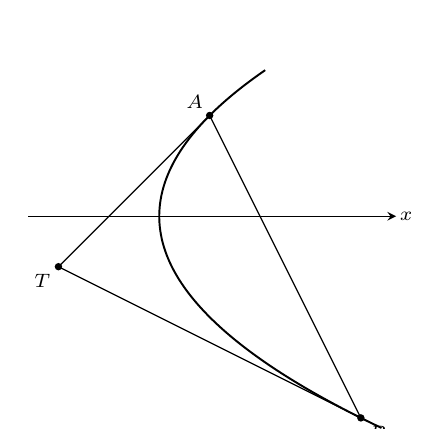
\begin{tikzpicture}[scale=1.28]
  \draw[caxis] (-1.3,0)--(2.35,0) node[clab,right]{$x$};
  \draw[ccurve,domain=-2.1:1.45,samples=90,smooth,variable=\t]
     plot ({0.5*\t*\t},{\t});
  \coordinate (A) at (0.5,1);
  \coordinate (B) at (2,-2);
  \coordinate (T) at (-1,-0.5);
  \draw[ctan] (A)--(T); \draw[ctan] (B)--(T);
  \draw[cseg] (A)--(B);
  \fill (A) circle (1.05pt) node[clab,above left=1pt]{$A$};
  \fill (B) circle (1.05pt) node[clab,below right=1.5pt]{$B$};
  \fill (T) circle (1.05pt) node[clab,below left=1.5pt]{$T$};
\end{tikzpicture} &
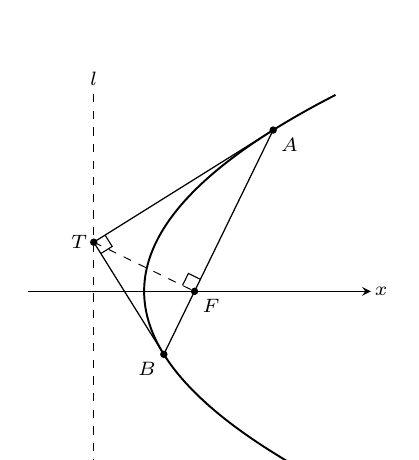
\begin{tikzpicture}[scale=1.28]
  \draw[caxis] (-1.15,0)--(2.25,0) node[clab,right]{$x$};
  \draw[ccurve,domain=-1.8:1.95,samples=80,smooth,variable=\t]
     plot ({0.5*\t*\t},{\t});
  \draw[caux] (-0.5,-1.75)--(-0.5,2.0) node[clab,above]{$l$};
  \coordinate (A) at (1.28,1.6);
  \coordinate (B) at (0.1953,-0.625);
  \coordinate (T) at (-0.5,0.4875);
  \coordinate (F) at (0.5,0);
  \draw[ctan] (A)--(T); \draw[ctan] (B)--(T);
  \draw[cseg] (A)--(B);
  \fill (A) circle (1.05pt) node[clab,below right=1.5pt]{$A$};
  \fill (B) circle (1.05pt) node[clab,below left=1.5pt]{$B$};
  \fill (T) circle (1.05pt) node[clab,left=1pt]{$T$};
  \fill (F) circle (1.05pt) node[clab,below right=1.5pt]{$F$};
  \draw pic[draw,angle radius=1.7mm] {right angle=A--T--B};
  \draw pic[draw,angle radius=1.7mm] {right angle=A--F--T};
  \draw[caux] (T)--(F);
\end{tikzpicture}\\
{\scriptsize (a) 一般情形} & {\scriptsize (b) $t_1t_2=-1$：$T$ 在准线上，$TA\perp TB$}
\end{tabular}
\caption{过 $A,B$ 的两条切线交于 $T$；垂直时交点落在准线上}
\end{figure}

\subsection{弦方程与弦中点}

若弦端点为 $A(\frac p2t_1^2,pt_1)$、$B(\frac p2t_2^2,pt_2)$，则
\[
\boxed{(t_1+t_2)y=2x+pt_1t_2}.
\]
设弦中点为 $M(x_M,y_M)$，则
\[
x_M=\frac p4(t_1^2+t_2^2),\qquad y_M=\frac p2(t_1+t_2).
\]
从而
\[
\boxed{k_{AB}=\frac{p}{y_M}},\qquad
\boxed{y_Mk_{AB}=p}.
\]
这条公式是抛物线中点弦问题的高频结论；当 $y_M=0$ 时弦为竖直弦，斜率不存在，需单独处理。

\subsection{焦点弦：参数乘积、长度与倒数和}

弦 $AB$ 过焦点 $F$ 的充要条件为
\[
\boxed{t_1t_2=-1}.
\]
因此焦点弦端点坐标满足
\[
\boxed{x_1x_2=\frac{p^2}{4},\qquad y_1y_2=-p^2}.
\]
焦点弦长为
\[
\boxed{AB=\frac p2(t_1-t_2)^2}.
\]
若焦点弦与对称轴夹角为 $\theta$（$\theta\ne0$），则
\[
\boxed{\{AF,BF\}=\left\{\frac{p}{1-\cos\theta},\frac{p}{1+\cos\theta}\right\}},
\]
\[
\boxed{\frac1{AF}+\frac1{BF}=\frac2p}.
\]
由 §2.12 的焦点弦长公式又得
\[
\boxed{AB\ge2p},
\]
等号在焦点弦垂直于对称轴（通径）时取得。

\subsection{焦点弦中点轨迹}

若 $M(x_M,y_M)$ 是焦点弦 $AB$ 的中点，则 $t_1t_2=-1$，于是
\[
x_M=\frac p4\big((t_1+t_2)^2-2t_1t_2\big)
=\frac p2+\frac p4(t_1+t_2)^2,\qquad
y_M=\frac p2(t_1+t_2).
\]
消去参数得
\[
\boxed{y_M^2=p\left(x_M-\frac p2\right)}.
\]
即抛物线所有焦点弦的中点轨迹是一条以焦点 $F(p/2,0)$ 为顶点、开口向右的抛物线。

\begin{figure}[H]
\centering
\begin{tikzpicture}[scale=1.0]
  \draw[caxis] (-0.5,0)--(2.95,0) node[clab,right]{$x$};
  \draw[ccurve,domain=-2.25:2.25,samples=90,smooth,variable=\t]
     plot ({0.5*\t*\t},{\t});
  \draw[line width=0.4pt,black!45] (2.279,2.135)--(0.110,-0.468);
  \draw[line width=0.4pt,black!45] (0.110,0.468)--(2.279,-2.135);
  \draw[dashed,line width=0.6pt,domain=-1.28:1.28,samples=70,smooth,variable=\t]
     plot ({\t*\t+0.5},{\t});
  \node[clab] at (2.28,-1.28) {轨迹};
  \fill (1.194,0.834) circle (1.4pt);
  \fill (1.194,-0.834) circle (1.4pt);
  \fill (0.5,0) circle (1.05pt) node[clab,below left=1pt]{$F$};
\end{tikzpicture}
\caption{焦点弦的中点轨迹：以 $F$ 为顶点、开口向右的抛物线（虚线）}
\end{figure}

\subsection{从定点向抛物线引切线}

设定点 $Q(x_0,y_0)$，过 $Q$ 的非竖直切线斜率为 $k$。抛物线切线可写为
\[
y=kx+\frac{p}{2k}.
\]
代入 $Q$ 得
\[
\boxed{x_0k^2-y_0k+\frac p2=0}.
\]
当 $y_0^2-2px_0>0$ 时，两条切线斜率 $k_1,k_2$（有限斜率情形且 $x_0\ne0$）满足
\[
\boxed{k_1+k_2=\frac{y_0}{x_0},\qquad k_1k_2=\frac{p}{2x_0}}.
\]
判别式为 $y_0^2-2px_0$。若 $x_0=0$，其中一条切线可能是顶点处的竖直切线 $x=0$，不能只数有限斜率根；若 $Q$ 恰为顶点，则只有顶点切线 $x=0$。

\subsection{焦点弦的圆性质（常见综合题）}

设 $AB$ 为抛物线焦点弦，$A',B'$ 分别为 $A,B$ 在准线上的垂足，则有：
\begin{itemize}
\item 以 $AB$ 为直径的圆与准线相切；
\item 以 $AF$ 或 $BF$ 为直径的圆与直线 $x=0$（即 $y$ 轴、顶点处的切线）相切；
\item 以 $A'B'$ 为直径的圆与直线 $AB$ 相切，切点为焦点 $F$。
\end{itemize}
\begin{figure}[H]
\centering
\begin{tikzpicture}[scale=1.4]
  \draw[caxis] (-1.35,0)--(2.5,0) node[clab,right]{$x$};
  \draw[ccurve,domain=-1.45:2.0,samples=80,smooth,variable=\t]
     plot ({0.5*\t*\t},{\t});
  \draw[caux] (-0.5,-1.45)--(-0.5,1.95);
  \coordinate (A) at (1.125,1.5);
  \coordinate (B) at (0.2222,-0.6667);
  \coordinate (Ap) at (-0.5,1.5);
  \coordinate (Bp) at (-0.5,-0.6667);
  \coordinate (F) at (0.5,0);
  \draw[cseg] (A)--(B);
  \draw[caux] (A)--(Ap); \draw[caux] (B)--(Bp);
  \node[clab] at (0.88,1.70) {$A$};
  \fill (A) circle (1.05pt);
  \fill (B) circle (1.05pt) node[clab,below left=2pt]{$B$};
  \fill (Ap) circle (1.05pt) node[clab,above left=1pt]{$A'$};
  \fill (Bp) circle (1.05pt) node[clab,below left=1.5pt]{$B'$};
  \fill (F) circle (1.05pt) node[clab,below=2pt]{$F$};
  \coordinate (Lu) at (-0.5,1.0);
  \coordinate (Ld) at (-0.5,-0.2);
  \draw pic[draw,angle radius=1.6mm] {right angle=A--Ap--Lu};
  \draw pic[draw,angle radius=1.6mm] {right angle=B--Bp--Ld};
\end{tikzpicture}
\caption{焦点弦 $AB$ 及其在准线上的射影 $A',B'$（$AA'\perp l$，$BB'\perp l$）}
\end{figure}

这类结论适合处理圆与直线相切、垂直、投影及面积问题。使用时先画出 $A,B,F,A',B'$ 的位置关系，再决定采用圆周角还是距离公式。

\subsection{阿基米德三角形：一般弦与焦点弦的特殊性质}

由弦 $AB$ 与 $A,B$ 两点处的切线围成的三角形 $TAB$，称为抛物线的阿基米德三角形。设 $A,B$ 的参数为 $t_1,t_2$，$T$ 为两切线交点，$M$ 为弦 $AB$ 的中点，则
\[
M=\left(\frac p4(t_1^2+t_2^2),\frac p2(t_1+t_2)\right).
\]
因此
\[
\boxed{TM\parallel x\text{ 轴}},\qquad
\boxed{S_{\triangle TAB}=\frac{p^2}{8}\abs{t_1-t_2}^{3}}.
\]
即阿基米德三角形顶点到底边中点的中线平行于抛物线对称轴。

若 $AB$ 还是焦点弦，则 $t_1t_2=-1$，从而有一组非常强的结论：
\[
\boxed{T\text{ 在准线 }x=-p/2\text{ 上}},\qquad
\boxed{TA\perp TB},\qquad
\boxed{TF\perp AB},
\]
以及
\[
\boxed{TF^2=AF\cdot BF}.
\]
\begin{figure}[H]
\centering
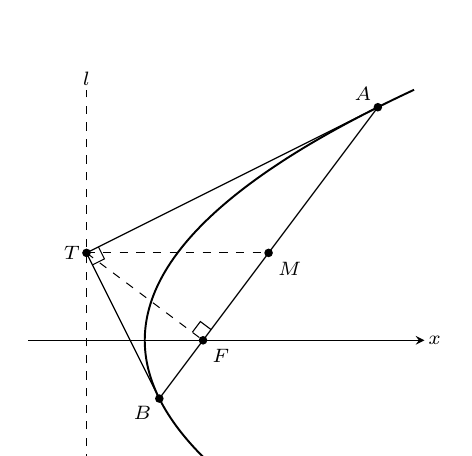
\begin{tikzpicture}[scale=1.48]
  \draw[caxis] (-1.0,0)--(2.4,0) node[clab,right]{$x$};
  \draw[ccurve,domain=-1.1:2.15,samples=80,smooth,variable=\t]
     plot ({0.5*\t*\t},{\t});
  \draw[caux] (-0.5,-1.05)--(-0.5,2.15) node[clab,above]{$l$};
  \coordinate (A) at (2,2);
  \coordinate (B) at (0.125,-0.5);
  \coordinate (T) at (-0.5,0.75);
  \coordinate (M) at (1.0625,0.75);
  \coordinate (F) at (0.5,0);
  \draw[ctan] (A)--(T); \draw[ctan] (B)--(T);
  \draw[cseg] (A)--(B);
  \draw[caux] (T)--(M);
  \draw[caux] (T)--(F);
  \fill (A) circle (1.05pt) node[clab,above left=1pt]{$A$};
  \fill (B) circle (1.05pt) node[clab,below left=1.5pt]{$B$};
  \fill (T) circle (1.05pt) node[clab,left=1pt]{$T$};
  \fill (M) circle (1.05pt) node[clab,below right=2pt]{$M$};
  \fill (F) circle (1.05pt) node[clab,below right=2pt]{$F$};
  \draw pic[draw,angle radius=1.7mm] {right angle=A--T--B};
  \draw pic[draw,angle radius=1.7mm] {right angle=A--F--T};
\end{tikzpicture}
\caption{阿基米德三角形 $TAB$：$TM\parallel x$ 轴；焦点弦时 $TF^2=AF\cdot BF$}
\end{figure}

也就是说，焦点弦对应的阿基米德三角形是以 $T$ 为直角顶点的直角三角形，焦点 $F$ 是从直角顶点向斜边 $AB$ 所作高的垂足。该组性质在涉及圆、垂直、切线交点、焦半径乘积时尤其有用。

\end{document}
